\chapter{4 quandrants chopper}
\section{General Description}

The general schematic of the device is shown in the following figure:

\begin{figure}[h]
\centering

\includegraphics[width=\linewidth]{TP_H4Q/fig/TP_H4Q.png}
%\caption{Simplified internal control}
\end{figure}

The power supply $U_E$ is achieved by a three-phase rectification of the 50 Hz network, variable up to 400 V using an autotransformer, followed by a filtering capacitor of value $C$. The DC machine has independent excitation which will be kept constant with an excitation current equal to its nominal value.

The ``rectifier-chopper'' assembly is realized within an integrated SEMIKRON device equipped with an external control system allowing for synchronous or delayed complementary control on each of the two ``bridge arms.''

The control device generates PWM signals whose duty cycle can be controlled using a potentiometer or an external voltage $v(t)$ \textbf{between 0 and 5V}.

\newpage
\section{Preparation}

The chopper is controlled with the command signals $f_1$, $f_2$, $f_3$, and $f_4$ below.

\begin{enumerate}
\item Plot the evolution of the chopper output voltage $U_m(t)$ assuming that the input voltage $U_e(t)$ is perfectly constant.
\item Calculate the average value of $U_m(t)$ as a function of the input voltage $U_e$ (assumed constant) and $\alpha$.
\end{enumerate}

\begin{figure}[h]
\centering
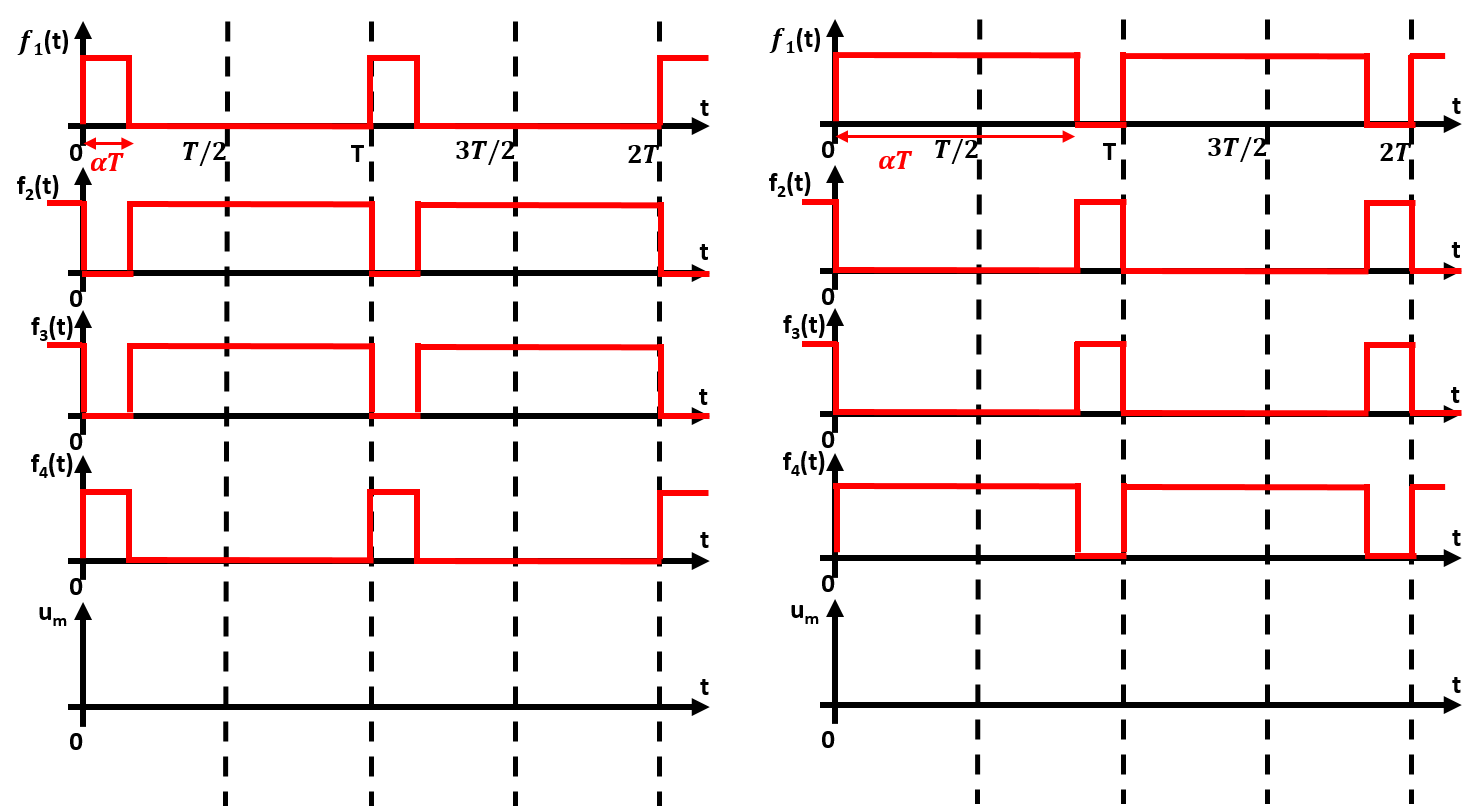
\includegraphics[width=1.1\linewidth]{TP_H4Q/fig/prepa_synchrone.png}
%\caption{Simplified internal control}
\end{figure}

\newpage
\section{Assembly Realization}

\begin{enumerate}
\item Record the characteristics of the DC machine and deduce the value of the rectified DC voltage $U_E$ necessary to exploit the entire speed range of this machine in both directions. This ``theoretical'' value of $U_E$ will be increased by 20\% to account for voltage drops and duty cycle limitations inherent to the control box.

\item Record the shape of the control signals labeled $COM$ and $\overline{COM}$ on the control box. (the $DEC$ and $\overline{DEC}$ signals will not be used) \textbf{Ensure that the duty cycle is different from 50\%}. Deduce:
\begin{itemize}
\item The connection of the control signals $COM$ and $\overline{COM}$
\item The shape of the chopper output voltage, particularly its amplitude and frequency.
\end{itemize}

\item Plot the control characteristic of this command, i.e., the duty cycle of the $COM$ command as a function of the external control voltage (\textbf{variable in the range 0 to 5V}). Deduce the value of this voltage that imposes the machine's stop.

\item Complete the assembly with the following recommendations:
\begin{itemize}
\item leave the DC machine unloaded;
\item if the machine has separate excitation, first connect its excitation and check the corresponding current value;
\item set the chopper control to impose a 50\% duty cycle;
\item gradually increase the network voltage (autotransformer) until the desired rectified voltage $U_E$ is reached;
\item test the proper functioning of the device by slowly varying the chopper control in both directions and continuously monitoring the motor armature current.
\end{itemize}

Since the assembly is quite ``voluminous'' to realize, care must be taken to wire the different blocks together in an easily verifiable manner. The various measuring devices must be readable, and the oscilloscope should be as far away as possible from the power connections.

\item If the motor braking is too fast, the DC bus voltage $U_E$ increases. Why? 

\underline{\textbf{In the presence of the instructor}}, observe this phenomenon.
\end{enumerate}

\section{Static Characterization of the Device}

\begin{enumerate}[label={}]
\item \textbf{Always ensuring that $U_E$ remains constant}, plot the chopper characteristic $<U_m>=f(\alpha)$, with the motor left unloaded ($\alpha$ represents the duty cycle of the $COM$ command). Carefully record the extreme possible duty cycle values, $\alpha_{min}$ and $\alpha_{max}$.
\end{enumerate}

\section{Dynamic Study of the Chopper}

In this study, a duty cycle of the type: $\alpha(t) = \alpha_0 + \Delta\alpha(t)$ is generated where $\Delta\alpha(t)$ is a ``slow'' variation and $\alpha_0 = 0.5$. For this, the control voltage used to drive the device includes a DC component $v_0$ and a low-frequency AC component, denoted $\Delta v(t)$. The motor will always be left unloaded \textbf{and care will be taken not to switch the functions of the control generator with a powered assembly} to avoid overcurrents.

\begin{enumerate}
\item Use the previous control characteristic to determine $v_0$ and $\Delta v(t)$ to vary the duty cycle linearly between 0.25 and 0.75. Gradually apply this voltage to the device (slowly increasing amplitude), at a cycle frequency of about 0.3 Hz (frequency of the $\Delta v$ signal).

\item Simultaneously record the motor armature current $i_M$ and the voltage measured by the tachogenerator $v_T$ (image of the speed $\Omega$). How to interpret these curves using the oscilloscope's XY mode (with sufficient persistence)? The measurement can be improved by inserting a low-pass filter on the current measurement to eliminate its ripple. How to choose the cutoff frequency of this filter?

\item Simultaneously observe the speed, the armature current, and the input voltage $U_e(t)$. Explain the variations observed on $U_e(t)$ and relate them to the 4 quadrants of operation.
\end{enumerate}

\section{Inverter}

Replace the motor with a series R - L load. We want to power this load with the North American electrical network (110V / 60 Hz) from our network (230V / 50 Hz). Therefore, we will use the chopper as a single-phase ``inverter'' to recreate this network. For this, a duty cycle of the form $\alpha(t) = \alpha_0 + \delta\alpha. sin(\omega t)$ will be used.
\begin{enumerate}
\item Determine $\alpha_0$, $\delta\alpha$, and $\omega$ to recreate the desired network.

\item Apply this control and power the load. Observe the output voltage $U_m$ of the chopper and $U_r$ the voltage across the resistor.
\end{enumerate}